\section{Simulations}

For all the simulations we set the physical parameters \(x_L = -1\), \(x_R = 1\), \(x_0 = -0.5\), \(\sigma_\textrm{norm} = 0.04\), \(n = 16\) and \(t_\textrm{fin} = 0.1\), unless specified otherwise. All physical values take arbitrary units as we imposed \(\hbar = 1\). We take \(n_x = 256\) mesh intervals and \(\Delta t = 10^{-4}\) for the numerical parameters, again unless specified otherwise.

\subsection{Infinite potential well}

In this section we will consider \(V_0 = 0\), which means that the particle is stuck in an infinite potential well as imposed by the border conditions. Let's first look at the propagation of a single particle and its properties.

\subsubsection{Physical properties}

\paragraph{General motion} The wave function, representing the probability distribution of finding the particle in a spatial interval, is shown in \autoref{fig:i_normpsi}. From this figure, we notice that the wave spreads out over time, and after hitting the potential wall gets reflected back. We observe an interesting phenomenon with this reflection: it seems that the wave gets reflected at different speeds, resulting in multiple peaks.

\begin{figure}[h]
    \centering
    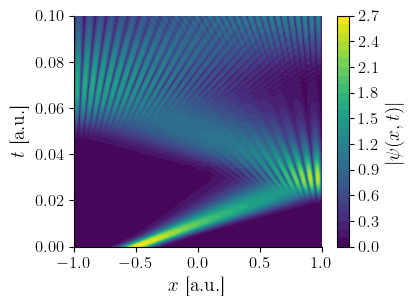
\includegraphics[width=0.6\linewidth]{figures/i_normpsi.png}
    \caption{Square root of the probability density of particle over space and time.}
    \label{fig:i_normpsi}
\end{figure}

\paragraph{Position and momentum} Now that we've seen the general "motion" of the particle, let's analyse some of its properties. Firstly, its average position is shown in \autoref{fig:i_xmoy}. We can se it initially moves as we would expect a classical particle to move (which we will compare later). When it reaches the right hand side border, it gets reflected and the average position seems to move a bit slower than before the reflection, before regaining the same speed. On the second bounce however, the average position seems to stabilise a bit, which is coherent with what we saw before: the reflections seperate the wave function in multiple thinner parts. The average position then doesn't mean very much, with the position being multiple similarly sized peaks. \autoref{fig:i_pmoy} shows the average momentum of the particle. The momentum remains constant before the particle "collides" with the wall, which is also what was observed with the constant average position change on the previous figure. After the collision, the sign of the momentum flips around, meaning the wave is moving left. It is not an abrupt change, as would be expected from a wave. After a second reflection, the average momentum doesn't seem to reach the initial momentum again. This could be explained because of the spreading of the wave, where on average the wave moves slower than initially.

\begin{figure}[h]
    \centering
    \begin{subfigure}{0.48\linewidth}
        \centering
        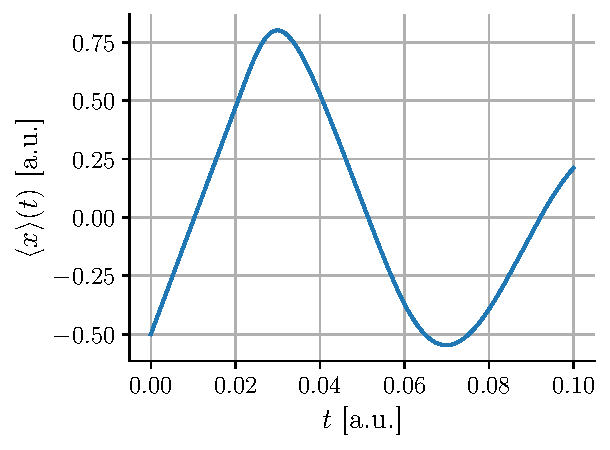
\includegraphics[width=\linewidth]{figures/i_xmoy.pdf}
        \caption{Average position}
        \label{fig:i_xmoy}
    \end{subfigure}
    \begin{subfigure}{0.48\linewidth}
        \centering
        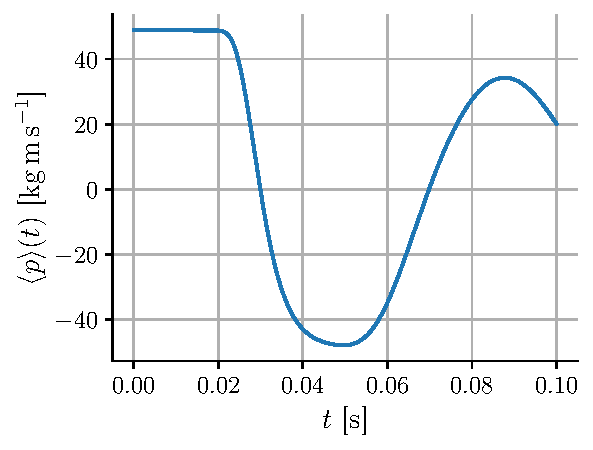
\includegraphics[width=\linewidth]{figures/i_pmoy.pdf}
        \caption{Average momentum}
        \label{fig:i_pmoy}
    \end{subfigure}
    \caption{Average position and momentum of a quantum particle in an infinite potential well}
    \label{fig:i_xmoy_pmoy}
\end{figure}

\paragraph{Uncertainty} For a quantum particle the uncertainty of its position and momentum is also a key property. \autoref{fig:i_deltax} shows the increasing uncertainty in position. It increases almost constantly, only decreasing when the wave change direction. On the momentum side, \autoref{fig:i_deltap} shows the uncertainty in momentum. As opposed to the position spread, the uncertainty in momentum increases sharply at the times when the wave is reflected, increasing from less than 10 a.u. to about 50 a.u., before decreasing again to about 10 a.u.. Every reflection increases the spread of momentum. This will be further commented on when looking at the Heisenberg uncertainty principle.

\begin{figure}[h]
    \centering
    \begin{subfigure}{0.48\linewidth}
        \centering
        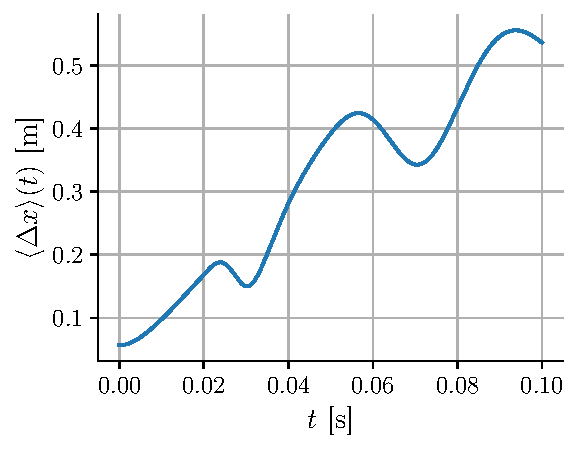
\includegraphics[width=\linewidth]{figures/i_deltax.pdf}
        \caption{Position spread}
        \label{fig:i_deltax}
    \end{subfigure}
    \begin{subfigure}{0.48\linewidth}
        \centering
        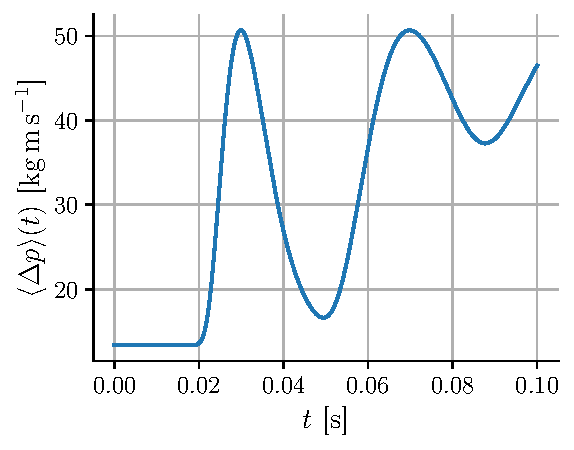
\includegraphics[width=\linewidth]{figures/i_deltap.pdf}
        \caption{Momentum spread}
        \label{fig:i_deltap}
    \end{subfigure}
    \caption{Spread over time of the position and momentum of a quantum particle in an infinite potential well}
    \label{fig:i_deltax_deltap}
\end{figure}

\paragraph{Group and phase velocity} Looking at the real part of the wave in \autoref{fig:i_repsi} allows us to notice a difference between the phase and group velocity. Indeed, we notice that peaks move along a slightly different path than the probability density shown before, meaning that the phase velocity is different to the group velocity. The phase velocity can be read with the slope of the peaks of the real part, using \(\dd x / \dd t = v\). From this we see that phase velocity is slower than the group velocity, as the slope \(\dd x / \dd t\) of the peak of the probability density is greater than that of the real part. The waves with slightly different initial velocities also split appart, resulating in the effect seen in \autoref{fig:i_normpsi} before. The speed of the peaks of the real part of the wave also decrease when approaching the walls, as can be seen by the slight curvature of the peak lines.

\begin{figure}[h]
    \centering
    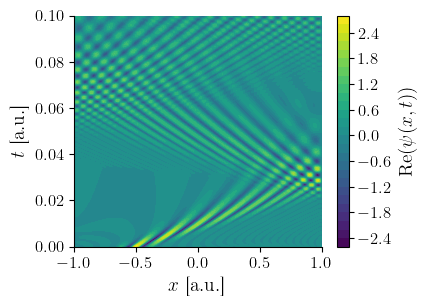
\includegraphics[width=0.6\linewidth]{figures/i_repsi.png}
    \caption{feur}
    \label{fig:i_repsi}
\end{figure}

\subsubsection{Comparing with classical particle}

It is also interesting to compare a quantum particle with a classical particle sharing some physical properties. First looking at a particle starting with the same initial energy as the quantum particle, i.e. staring with a speed
\begin{equation}
    E = \frac{p^2}{2m} \stackrel{m=1,\ p=mv}{\implies} v = \pm \sqrt{2E}
\end{equation}
we obtain the movement shown in \autoref{fig:i_classical_vs_quantum_energy}. We chose the positive solution as we want both particles to move in the same direction initially. The same was done for a particle sharing the same initial momentum as the quantum particle, shown in \autoref{fig:i_classical_vs_quantum_momentum}. We notice that the particle sharing the same energy moves faster than the particle sharing the same initial momentum. The faster particle also doesn't match the quantum particle's average position, even before the first bounce, while the slower one matches the average position exactly, except at the borders. An interesting thing to note is that the classical particle with same momentum intersects with the average position of the quantum particle exactly at \(x=0\). From these observations we can deduce that there must be another component than the momentum contributing to the energy of the quantum particle, which is not the potential because it was set to 0.

\begin{figure}[h]
    \centering
    \begin{subfigure}{0.48\linewidth}
        \centering
        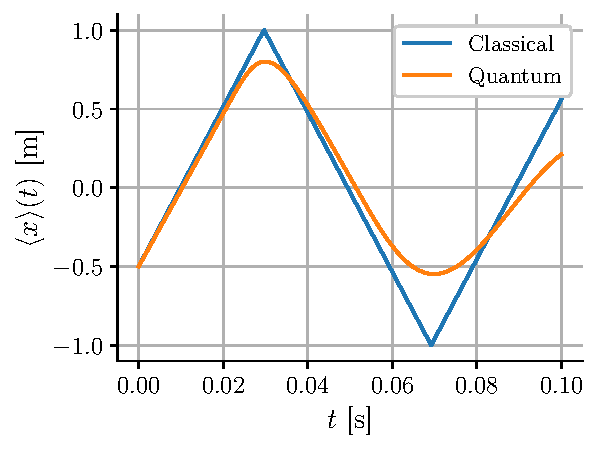
\includegraphics[width=\linewidth]{figures/i_classical_vs_quantum_energy.pdf}
        \caption{Same energy}
        \label{fig:i_classical_vs_quantum_energy}
    \end{subfigure}
    \begin{subfigure}{0.48\linewidth}
        \centering
        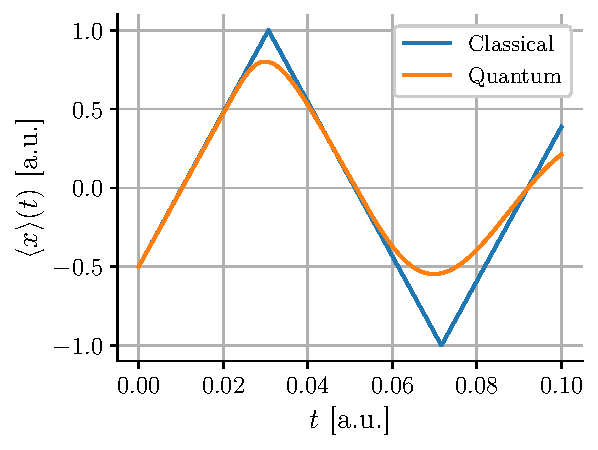
\includegraphics[width=\linewidth]{figures/i_classical_vs_quantum_momentum.pdf}
        \caption{Same initial momentum}
        \label{fig:i_classical_vs_quantum_momentum}
    \end{subfigure}
    \caption{feur}
    \label{fig:i_classical_vs_quantum}
\end{figure}

\subsubsection{Verifying properties of the Crank-Nocloson method}

Let's also verify features of the the Crank Nicolson method. Firstly, it was shown in the book \cite{physnumbook} that this method conserves energy to machine precision. This phenomenon can clearly be seen in \autoref{fig:i_conservation_energy}, with the stairs clearly showing errors due to floating point approximations. The error on energy conservation was found to be on the order of \(10^{-10}\). This method is also supposed to conserve normalisation (i.e. probability), which is shown in \autoref{fig:i_conservation_probability}. It is clear that the total probability remains constant, at \(1\). Due to the smaller values of probability, the error on conservation of probability was found to be on the order of \(10^{-13}\).

\begin{figure}[h]
    \centering
    \begin{subfigure}{0.55\linewidth}
        \centering
        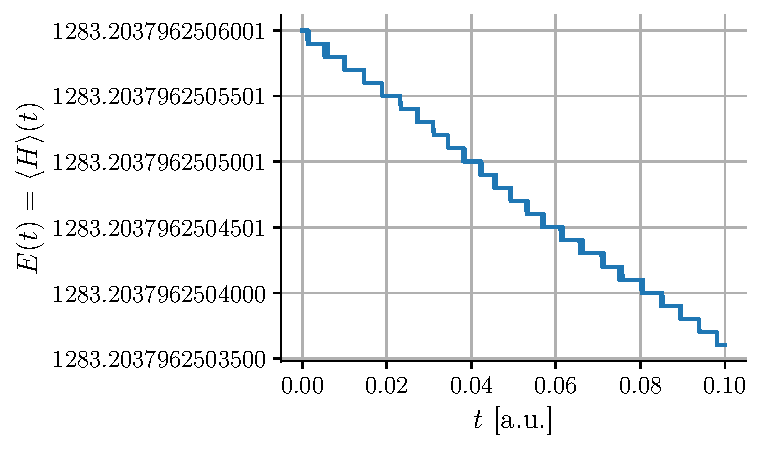
\includegraphics[width=\linewidth]{figures/i_conservation_energy.pdf}
        \caption{Energy of particle}
        \label{fig:i_conservation_energy}
    \end{subfigure}
    \begin{subfigure}{0.44\linewidth}
        \centering
        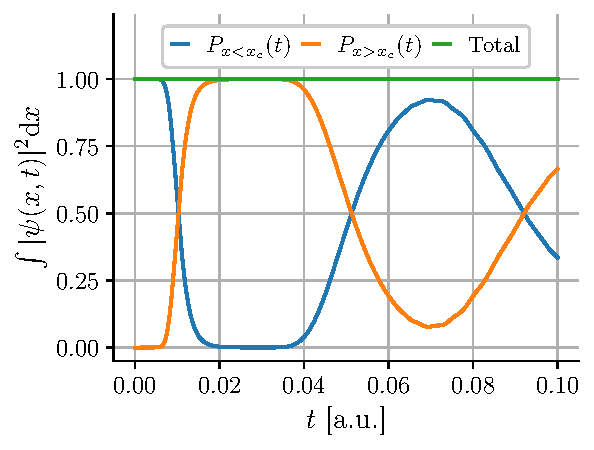
\includegraphics[width=\linewidth]{figures/i_conservation_probability.pdf}
        \caption{Normalisation}
        \label{fig:i_conservation_probability}
    \end{subfigure}
    \caption{Conservation of the particle's physical properties}
    \label{fig:i_conservation}
\end{figure}

\paragraph{Heisenberg uncertainty principle} Finally, we want to verify that the simulation produces sane physical results, more specifically that it follows the Heisenberg uncertainty principle. With our unit normalisation, this corresponds to:
\begin{equation}
    \langle \Delta x \rangle \langle \Delta p \rangle \ge \frac{1}{2}
\end{equation}
The results from the simulation are shown in \autoref{fig:i_heisenberg}. The minimal value for the product \(\langle \Delta x \rangle \langle \Delta p \rangle\) is around \(0.75\). We conclude that the Heisenberg uncertainty principle is respected. We notice that the product increases over time, meaning that we know less and less where the particle is and what momentum it has, as was seen previously.

\begin{figure}[h]
    \centering
    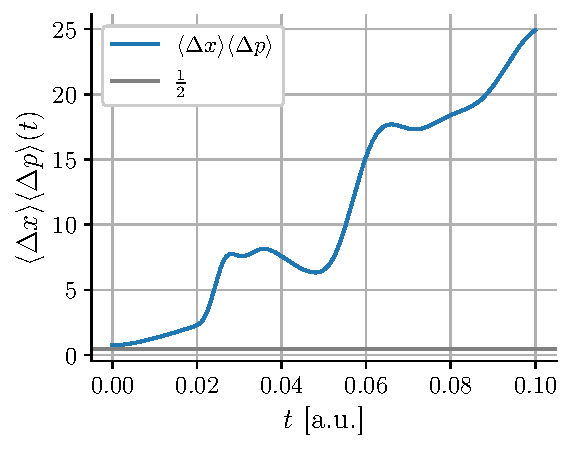
\includegraphics[width=0.6\linewidth]{figures/i_heisenberg.pdf}
    \caption{Verification of Heisenberg's uncertainty principle}
    \label{fig:i_heisenberg}
\end{figure}

\subsection{Well well well if it isnt the double potential well}

feur all over heisenberg
